%
% File naaclhlt2012.tex
%

\documentclass[11pt,letterpaper]{article}
\usepackage{naaclhlt2012}
\usepackage{times}
\usepackage{latexsym}
\usepackage{amsmath}
\usepackage{graphicx}
\setlength\titlebox{6.5cm}    % Expanding the titlebox

\title{Tackling Dialog State Tracking Challenge}

\author{Wencan Luo\\
	    Department of Computer Science\\
	    University of Pittsburgh\\
	    PA 15260, USA\\
	    {\tt wencan@cs.pitt.edu}
	  }

\date{September 9, 2013}

\begin{document}
\maketitle
\begin{abstract}
We will propose a model to tackle the Dialog State Tracking Challenge \cite{Williams:2013a}.

\end{abstract}

\section{Introduction}
In dialog systems, ``state tracking" refers to accurately estimating the user�s goal as a dialog progresses. Accurate state tracking is desirable because it provides robustness to errors in speech recognition, and helps reduce ambiguity inherent in language within a temporal process like dialog. Dialog state tracking is an important problem for both traditional uni-modal dialog systems, as well as speech-enabled multi-modal dialog systems on mobile devices, on tablet computers, and in automobiles \cite{Williams:2012}. 

The 2013 ``Dialog State Tracking Challenge"(DSTC) provided a good test bank for this task. This challenge has completed. 9 teams entered a total of 27 entries. Results have been shown at SigDial 2013.

However, the data is still public available\footnote{http://research.microsoft.com/en-us/events/dstc/. This link was broken a few days ago, but it is fixed up after a request}.

\section{Task Description}
DSTC data is taken from several different spoken dialog systems. All of them provide bus schedule information for Pittsburgh, Pennsylvania, USA \cite{Black:2011}. Different dialog systemw might have different ASR, NLU and dialog control components. In this challenge, only 9 slots are evaluated: route, from.desc, from.neighborhood, from.monument, to.desc, to.neighborhood, to.monument, date, and time. The approximate numbers of distinct values for slots are shown in Table \ref{table:slot_num}. The number of values for each slot varies a lot.

The dialog systems logged SLU N-best hypotheses for each user turn with confidence scores. As they claimed, the coverage of N-best hypotheses is good, so the challenge confines consideration of goals to slots and values that have been observed in an SLU output. The task of a dialog state tracker is to generate a set of observed slot and value pairs, with a score between 0 and 1. The sum of all scores should be 1. In which, the correct slot value should have maximal value.

For evaluation, there are 11 different metrics, 4 test tests under 3 different schedules \cite{Williams:2013a} for 9 slots.

\begin{table}[!htb] 
\centering
\begin{tabular}{c|c}
Slot name& number of values\\\hline
route&100\\
from.desc&500-10000\\
to.desc&500-10000\\
from.neighborhood&20-100\\
to.neighborhood&20-100\\
from.monument&50-500\\
to.monument&50-500\\
date.day&9\\
date.absmonth&12\\
date.absday&31\\
date.relweek&1\\
time.hour&12\\
time.minute&60\\
time.ampm&2\\
time.arriveleave&2\\
time.rel&1\\
\end{tabular}
\caption{Approximate number of distinct values for slots}
\label{table:slot_num}
\end{table}

\section{The Corpus}
The data is divided into 4 training sets and 4 test sets. They come from different sources. The basic statistical information for the corpus is shown in Table \ref{table:corpus}

\begin{table*}[!htb]
\centering
\begin{tabular}{l|c|c|c|c}
Role&PM&ME&UI&ID\\\hline
Ratio&36.6\%&22.1\%&19.8\%&21.5\%\\
\end{tabular}

\caption{Dataset description}
\label{table:corpus}
\end{table*}

\section{Related Work}
\subsection{Overall Results}

9 teams entered the DSTC, submitting a total of 27 trackers.

Here is the summary of the results \cite{Williams:2013a}.

Firstly, relative 
to the baselines, performance on the test data is
markedly lower than the training data. Moreover, only 38\% of trackers performed
better than a simple majority-class baseline on TEST4.

Secondly, no one wins. Different trackers are tuned for different performance measures, and the optimal tracking algorithm depends crucially on the target performance measure. The average rank of entries for four metrics is shown in Figure \ref{fig:ranking}.

\begin{figure}[!htb]
\centering
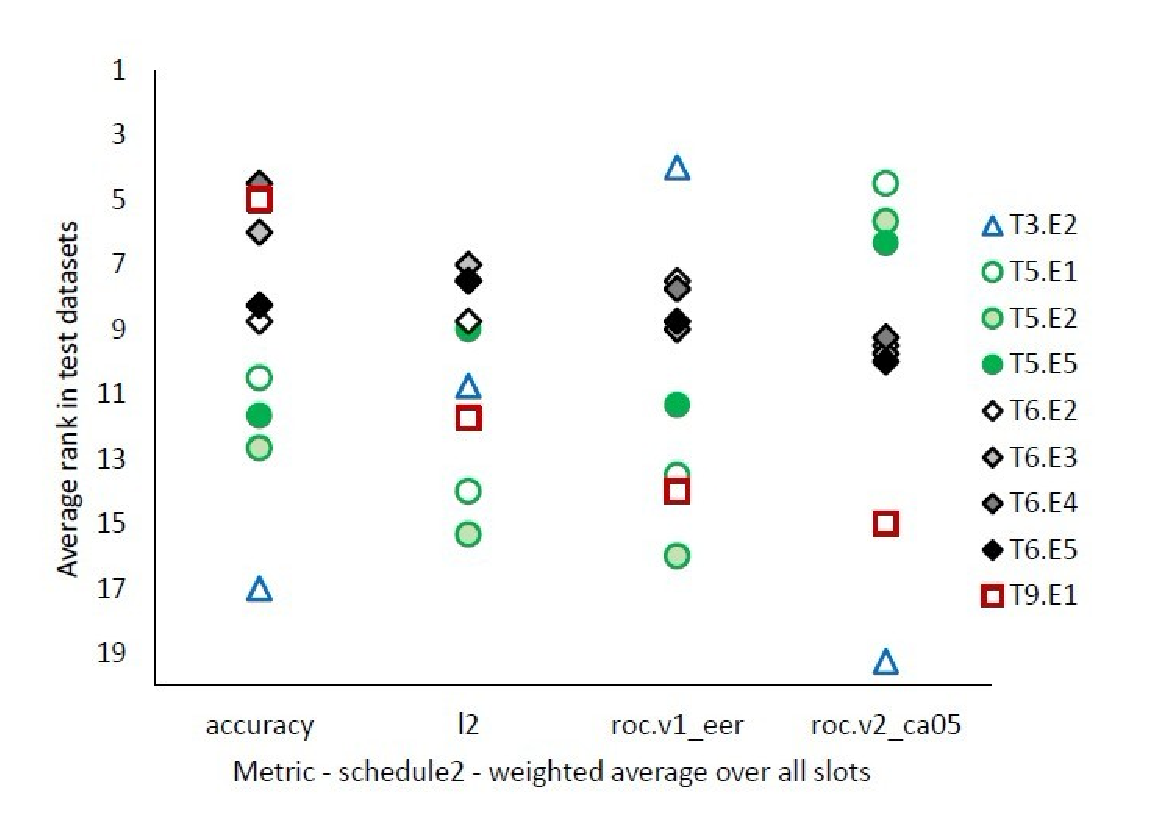
\includegraphics[width=80mm]{ranking.eps}
\caption{Average rank of top-performing trackers for four metrics. Ranking 
was done using the given metric, schedule2,
and the weighted average of all slots. $Tn.Em$ indicates team $n$, entry $m$.}
\label{fig:ranking}
\end{figure}

\subsection{Methodology}

The methods are briefly summarized in Table \ref{table:methods}.
\begin{table*}[!htb] 
\centering
\begin{tabular}{l|l|l|l}
Team&Author&Method&New Ideas\\\hline
1&\cite{Metallinou:2013}&MaxEnt&speech recognition error pattern\\
2&\cite{Henderson:2013}&Deep Neural Network&deep learning\\
3&\cite{Cuayahuitl:2013}&Bayesian Networks&re-ranking N-best ASR\\
4&\cite{Lee:2013a}&MaxEnt&L1 regularization, bins\\
&\cite{Lee:2013b}&Structured Discriminative model&\\
5&\cite{Wang:2013}&Rules&infor, deny, affirm, negate\\
6&\cite{Williams:2013b}&MaxEnt&multi-domain learning\\
7&\cite{Zilka:2013}&Bayesian, Generative&\\
8&\cite{Ren:2013}&CRF&\\
9&\cite{Kim:2013}&Different models&\\
\end{tabular}
\caption{Different approaches submitted  by the participants\footnote{The ID of the teams are not necessary as the same as shown in Figure \ref{fig:ranking}}}
\label{table:methods}
\end{table*}

Generally speaking, these methods are trying to rescore ASR/NLU engines, but not trying to consider the semantic meaning of the sentences. Commonly features are the rank of NLU slots, the rank of ASR, etc.

Here are some ideas that have not been tried in their reports.

\begin{itemize}
  \item re-run the NLU
  \item take the bus schedule into account (the schedule has been given)
  \item try to really understand the conversation between the computer and the human (Graph Model?)
\end{itemize}

\section{Timeline}

\noindent \emph{Sep 15 - Sep 22}
\begin{itemize}
  \item survey the related work regarding dialog state tracking
  \item understanding the data, know how to extract and use the data
\end{itemize}

\noindent \emph{Sep 23 -  Oct 20}
\begin{itemize}
  \item implement discriminative model used the basic features introduced in the SigDial 2013 reports
\end{itemize}

\noindent \emph{Oct 21 - Nov 9}
\begin{itemize}
  \item re-run NLU using CRF model
  \item combined the new NLU with the old NLU
\end{itemize}

\noindent \emph{Nov 10 - Dec 12}
\begin{itemize}
  \item do error analysis and propose new features and/or new model for this task
\end{itemize}

\section*{Acknowledgments}

Do not number the acknowledgment section.

\begin{thebibliography}{}

\bibitem[\protect\citename{Williams et al.}2012]{Williams:2012}
J. D. Williams, A. Raux, D. Ramachandran, and A. W. Black.
\newblock 2012. 
\newblock {\em Dialog state tracking challenge handbook}. 
\newblock Technical report, Microsoft Research.

\bibitem[\protect\citename{Williams et al.}2013]{Williams:2013a}
J. D. Williams, A. Raux, D. Ramachandran, and A. W. Black.
\newblock 2013. 
\newblock {\em The Dialog State Tracking Challenge}. 
\newblock In Proceedings 14th Annual Meeting of the Special Interest Group on Discourse and Dialogue (SIGDIAL), Metz, France. 

\bibitem[\protect\citename{Williams}2013]{Williams:2013b}
J. Williams.
\newblock 2013. 
\newblock {\em Multi-domain learning and generalization in dialog state tracking}. 
\newblock In Proceedings 14th Annual Meeting of the Special Interest Group on Discourse and Dialogue (SIGDIAL), Metz, France. 

\bibitem[\protect\citename{Black et al.}2013]{Black:2011}
A. Black et al.
\newblock 2011. 
\newblock {\em Spoken dialog challenge 2010: Comparison of live and control test results}. 
\newblock In Proceedings of SIGDIAL.

\bibitem[\protect\citename{Cuayahuitl et al.}2013]{Cuayahuitl:2013}
H. Cuayahuitl, N. Dethlefs, H. Hastie, O. Lemon.
\newblock 2013. 
\newblock {\em Impact of ASR N-Best Information on Bayesian Dialogue Act Recognition}. 
\newblock In Proceedings of SIGDIAL.

\bibitem[\protect\citename{Henderson et al.}2013]{Henderson:2013}
M. Henderson, B. Thomson and S. Young.
\newblock 2013. 
\newblock {\em Deep Neural Network Approach for the Dialog State Tracking Challenge}. 
\newblock In Proceedings 14th Annual Meeting of the Special Interest Group on Discourse and Dialogue (SIGDIAL), Metz, France. 

\bibitem[\protect\citename{Kim et al.}2013]{Kim:2013}
D. Kim, J. Choi, K. E. Kim, J. Lee and J. Sohn.
\newblock 2013. 
\newblock {\em Engineering Statistical Dialog State Trackers: A Case Study on DSTC}. 
\newblock In Proceedings 14th Annual Meeting of the Special Interest Group on Discourse and Dialogue (SIGDIAL), Metz, France. 

\bibitem[\protect\citename{Lee and Eskenazi}2013]{Lee:2013a}
S. Lee and M. Eskenazi.
\newblock 2013. 
\newblock {\em Recipe For Building Robust Spoken Dialog State Trackers: Dialog State Tracking Challenge System Description}. 
\newblock In Proceedings 14th Annual Meeting of the Special Interest Group on Discourse and Dialogue (SIGDIAL), Metz, France. 

\bibitem[\protect\citename{Lee}2013]{Lee:2013b}
S. Lee.
\newblock 2013. 
\newblock {\em Structured Discriminative Model For Dialog State Tracking}. 
\newblock In Proceedings 14th Annual Meeting of the Special Interest Group on Discourse and Dialogue (SIGDIAL), Metz, France. 

\bibitem[\protect\citename{Metallinou et al.}2013]{Metallinou:2013}
A. Metallinou, D. Bohus, and J. D. Williams
\newblock 2013. 
\newblock {\em Discriminative state tracking for spoken dialog systems}. 
\newblock In Proceedings 14th Annual Meeting of the Special Interest Group on Discourse and Dialogue (SIGDIAL), Metz, France. 

\bibitem[\protect\citename{Ren et al.}2013]{Ren:2013}
H. Ren, W. Xu, Y. Zhang and Y. Yan.
\newblock 2013. 
\newblock {\em Dialog State Tracking using Conditional Random Fields}. 
\newblock In Proceedings 14th Annual Meeting of the Special Interest Group on Discourse and Dialogue (SIGDIAL), Metz, France. 

\bibitem[\protect\citename{Wang and Lemon}2013]{Wang:2013}
Z. Wang and O. Lemon.
\newblock 2013. 
\newblock {\em A Simple and Generic Belief Tracking Mechanism for the Dialog State Tracking Challenge: On the believability of observed information}. 
\newblock In Proceedings 14th Annual Meeting of the Special Interest Group on Discourse and Dialogue (SIGDIAL), Metz, France. 

\bibitem[\protect\citename{Zilka et al.}2013]{Zilka:2013}
L. Zilka, D. Marek, M. Korvas and F. Jurcicek.
\newblock 2013. 
\newblock {\em Comparison of Bayesian Discriminative and Generative Models for Dialogue State Tracking}. 
\newblock In Proceedings 14th Annual Meeting of the Special Interest Group on Discourse and Dialogue (SIGDIAL), Metz, France. 

\end{thebibliography}

\end{document}
